\begin{figure*}[]
    \centering  
    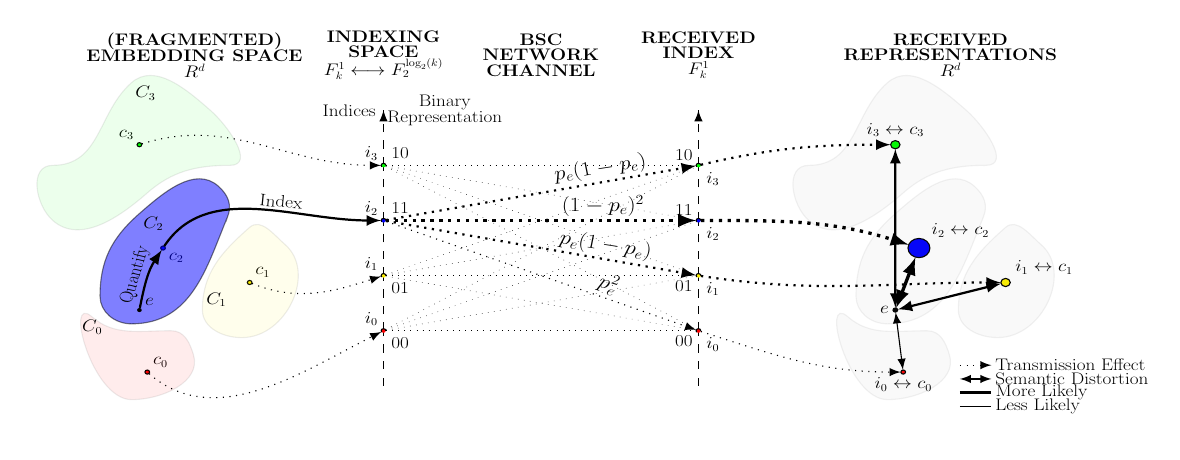
\begin{tikzpicture}[xscale=0.4,yscale=0.35,every node/.style={transform shape,font=\fontsize{16pt}{16pt}\selectfont},bullet/.style={circle,fill,inner sep=1.5pt,node contents={}}] %every node/.style={scale=0.9}]
        \contourlength{1.4pt}
        \tikzset{>=latex} % for LaTeX arrow head
        %Manually reduce line spacing to single space no matter double or single column document (draft mode)
        \linespread{1}
        
        % \draw (0,0) node[bullet,label=left:$P_C(x)$,alias=PC]  -- (15:3) coordinate[midway] (aux)
        % node[bullet,label=above right:$x$] -- ++ (-145:4.5) node[midway,below right]{$\|x-z\|$}     node[bullet,label=below left:$z$];
        % \draw (PC) to[out=105,in=0] ++ (-0.75,1) to[out=180,in=105] ++ (-1.5,-3)
        % node[above right]{$C$} to[out=-75,in=180] ++ (1.25,-1) to[out=0,in=-75] cycle;
        % \draw[shorten <=2pt,-latex] (aux) to[out=90,in=-90] ++ (110:0.8) node[above]{$\|x-P_C(x)\|$};

        % % EMBEDDING SPACE
        % \draw (0,0) node[alias=C0] { } ++(-1.5,-0.5) coordinate[midway] (aux) node[bullet,fill=red,draw,label=above right:$c_0$, alias=X0];
        % \draw [fill=red,opacity=0.075] (C0) to[out=105,in=0] ++ (-0.75,1) to[out=180,in=315] ++ (-2.5,+0.5) node[opacity=1,below]{$C_0$} to[out=135,in=180] ++ (1.25,-3) to[out=0,in=-75] cycle;

        % \draw (3,4) node[alias=C1] { } ++(-1.25,-1.25) coordinate[midway] (aux) node[bullet,fill=yellow,draw,label=above right:$c_1$, alias=X1];
        % \draw [fill=yellow,opacity=0.075] (C1) to[out=135,in=45] ++ (-1.25,+0.75) to[out=225,in=90] ++ (-1.5,-3) node[opacity=1,above right]{$C_1$} to[out=270,in=180] ++ (1.25,-1) to[out=0,in=315] cycle;

        % \draw (1,5) node[alias=C2] { } ++(-2,-1) coordinate[midway] (aux) node[bullet,fill=blue,draw,label=below right:$c_2$, alias=X2];;
        % \draw [fill=blue,opacity=0.5,draw=black] (C2) to[out=70,in=315] ++ (-0.25,1.25) to[out=135,in=45] ++ (-2.5,-1) node[opacity=1,below right]{$C_2$} to[out=225,in=90] ++ (-1.25,-3) to[out=270,in=180] ++ (+1,-1) to[out=0,in=250]cycle;

        % \draw (+1,+7) node[alias=C3] { } ++(-2.75,+0.75) coordinate[midway] (aux) node[bullet,fill=green,draw,label=above left:$c_3$, alias=X3];
        % \draw [fill=green,opacity=0.075] (C3) to[out=0,in=315] ++ (-0.5,+2) to[out=135,in=45] ++ (-2.5,+1) node[opacity=1,below right]{$C_3$} to[out=225,in=0] ++ (-2.5,-3) to[out=180,in=135] ++ (+0,-2) to[out=315,in=225] ++ (+3,+1) to[out=45,in=180]cycle;

        % % INDEX SPACE
        % \draw [->, dashed] (+5,-1) node[alias=axis_begin] {}  -- ++(+0,+2) coordinate[midway] (aux) node[bullet,fill=red,draw,label=above left:$i_0$,alias=I0] ++ (0,0) node[label=below right:$00$] {}-- ++(+0,+2) coordinate[midway] (aux) node[bullet,fill=yellow,draw,label=above left:$i_1$,alias=I1] ++ (0,0) node[label=below right:$01$] {}-- ++(+0,+2) coordinate[midway] (aux) node[bullet,fill=blue,draw,label=above left:$i_2$,alias=I2] ++ (0,0) node[label=below right:$11$] {}-- ++(+0,+2) coordinate[midway] (aux) node[bullet,fill=green,draw,label=above left:$i_3$,alias=I3] ++ (0,0) node[label=below right:$10$] {}-- ++(+0,+2) coordinate[midway] (aux) node[label=above left:Indices,alias=axis_end] {} ++ (0,0) node[above right, align=center] {Binary\\Representation};

        % \draw [<->,dotted] (X0) to[out=-45,in=225] (I0);
        % \draw [<->,dotted] (X1) to[out=-45,in=225] (I1);
        % \draw [->, thick] (X2) to[out=+65,in=150] node [above,pos=0.8, rotate=-20]  {Index} ++ (+4,+1) to[out=330,in=225](I2);
        % \draw [<->,dotted] (X3) to[out=+45,in=225] (I3);
        
        % % PHYSICAL REPRESENTATION
        % \node (QAMORIGIN) at (+9,+4) {};

        % \def\particles{(10.5,5.5)}
        % \foreach \point in \particles{
        %   \foreach\i in {0,0.01,...,1} { 
        %     \fill[opacity=0.1*\i,gray,rotate around={30:\point}] \point ellipse ({3-3*\i} and {3-3*\i});         
        %   }
        %   %\fill[black] \point circle (2mm);
        % } 
        % \draw (QAMORIGIN) ++ (2.5,2.5) node [rotate=0, align=center] {Gaussian\\Noise};
        % \draw [->] (QAMORIGIN) ++ (-2.5,0) -- ++(+5,+0) node [above] {I}; 
        % \draw [->] (QAMORIGIN) ++ (0,-2.5) -- ++(+0,+5) node [right] {Q}; 

        % \draw (QAMORIGIN) ++ (-1.5,-1.5) node[bullet,fill=red,draw,label=above right:$s_0$, alias=S0];
        % \draw (QAMORIGIN) ++ (-1.5,1.5) node[bullet,fill=yellow,draw,label=below right:$s_1$, alias=S1];
        % \draw (QAMORIGIN) ++ (1.5,1.5) node[bullet,fill=blue, draw,label=below left:$s_2$, alias=S2];
        % \draw (QAMORIGIN) ++ (1.5,-1.5) node[bullet,fill=green,draw,label=above left:$s_3$, alias=S3];

        % \draw [<->,dotted] (I0) to[out=45,in=160] (S0);
        % \draw [<->,dotted] (I1) to[out=45,in=180] (S1);
        % \draw [->, thick] (I2) to[out=45,in=90] node [above,pos=0.4,rotate=20] {Map} (S2);
        % \draw [<->,dotted] (I3) to[out=45,in=150] ++ (+7,+2) to[out=-30,in=0] (S3);

        % % EMBBEDINGS TRANSMISSION
        % \draw (-1.5,+1.5) coordinate[midway] (aux) node[bullet,label=above right:$e$, alias=E];
        % \draw [->,thick] (E) to[out=90,in=245] node [above,pos=0.5, rotate=80] {Quantify} (X2);

        % % RECEIVED REPRESENTATIONS
        % \node (RR) at (+19,+0) {};
        % % \draw (RR) ++ (0,0) ++ (-1.5,-0.5) node[bullet,inner sep= 1.5pt,label=below:$c_0$, alias=RX0];
        % % \draw (RR) ++ (3,4) ++ (-1.25,-1.25) node[bullet,inner sep= 3pt,label=above right:$c_1$, alias=RX1];
        % % \draw (RR) ++ (1,5) ++(-2,-1) node[bullet,inner sep= 5pt,label=above :$c_2$, alias=RX2];
        % % \draw (RR) ++ (+1,+7) ++(-2.75,+0.75) node[bullet,inner sep= 3pt, label=above left:$c_3$, alias=RX3];
        
        
        % \draw (RR) ++ (-1.5,+1.5) coordinate[midway] (aux) node[bullet,fill=black,draw,label=left:$e$, alias=RE];




        % \draw (RR) node[alias=RC0] { } ++(-1.5,-0.5) node[fill=red,draw,bullet,inner sep= 1.5pt,label=below:$s_0 \leftrightarrow c_0$, alias=RX0];
        % \draw [fill=gray,opacity=0.05] (RC0) to[out=105,in=0] ++ (-0.75,1) to[out=180,in=315] ++ (-2.5,+0.5) to[out=135,in=180] ++ (1.25,-3) to[out=0,in=-75] cycle;

        % \draw (RR) ++ (3,4) node[alias=RC1] { } ++ (-1.25,-1.25) node[fill=yellow,draw,bullet,inner sep= 3pt,label={below right,label distance=0.1cm,rotate=0}:$s_1 \leftrightarrow c_1$, alias=RX1];
        % \draw [fill=gray,opacity=0.05] (RC1) to[out=135,in=45] ++ (-1.25,+0.75) to[out=225,in=90] ++ (-1.5,-3) to[out=270,in=180] ++ (1.25,-1) to[out=0,in=315] cycle;

        % \draw (RR) ++ (1,5) node[alias=RC2] { } ++(-2,-1) node[fill=blue,draw,bullet,inner sep= 5pt,label={below right,label distance=1pt,rotate=0}:$s_2 \leftrightarrow c_2$, alias=RX2];
        % \draw [fill=gray,opacity=0.05] (RC2) to[out=70,in=315] ++ (-0.25,1.25) to[out=135,in=45] ++ (-2.5,-1) to[out=225,in=90] ++ (-1.25,-3) to[out=270,in=180] ++ (+1,-1) to[out=0,in=250]cycle;

        % \draw (RR) ++ (+1,+7) node[alias=RC3] { } ++(-2.75,+0.75) node[fill=green,draw,bullet,inner sep= 3pt, label=above:$s_3 \leftrightarrow c_3$, alias=RX3];
        % \draw [fill=gray,opacity=0.05] (RC3) to[out=0,in=315] ++ (-0.5,+2) to[out=135,in=45] ++ (-2.5,+1) to[out=225,in=0] ++ (-2.5,-3) to[out=180,in=135] ++ (+0,-2) to[out=315,in=225] ++ (+3,+1) to[out=45,in=180]cycle;

        
        % \draw [->, densely dashed] (RE) to[out=50,in=280] node [below,pos=0.5, rotate=60, align=center] {} (RX2);

        % \draw [->, very thick, densely dotted] (RX2) to[out=50,in=0] node [above,pos=0.8, rotate=0, align=center] {$\mathbb{P}\{s_2|s_2\}$} ++ (0,2) to[out=180,in=130] (RX2);
        % \draw [->, thick, densely dotted] (RX2) to[out=20,in=200] ++ (+2,+1.25) to[out=20,in=90] node [right,pos=0.5, rotate=0, align=center] {$\mathbb{P}\{s_1|s_2\}$} (RX1);
        % \draw [->, thick, densely dotted] (RX2) to[out=30,in=-80] ++ (+1.5,+2.5) to[out=100,in=0]  node [right,pos=0., rotate=0, align=center] {$\mathbb{P}\{s_3|s_2\}$} (RX3);
        % \draw [->, densely dotted] (RX2) to[out=180,in=135] node [left,pos=0.5, rotate=0, align=center] {$\mathbb{P}\{s_0|s_2\}$} (RX0);

        % \draw [<->, very thick] (RX2) -- node [below,pos=0.5, rotate=+23, align=center] {} (RE);
        % \draw [<->, thick] (RX1) -- node [below,pos=0.5, rotate=+23, align=center] {} (RE);
        % \draw [<->, thick] (RX3) -- node [above,pos=0.5, rotate=+93, align=center] {} (RE);
        % \draw [<->] (RX0) -- node [below,pos=0.55, rotate=+90, align=center] {} (RE);

        % % LEGENDS
        % \node (RRL) at (18.3,+1.25) {};
        % \draw [->, densely dashed] (RRL) ++ (1,-1) -- node [right,pos=1, rotate=0, align=center] {Quantification Error}++ (1,0) ;
        % \draw [->, densely dotted] (RRL) ++ (1,-1.5) -- node [right,pos=1, rotate=0, align=center] {Transmission Effect} ++ (1,0) ;
        % \draw [<->] (RRL) ++ (1,-2) -- node [right,pos=1, rotate=0, align=center] { Semantic Distortion}++ (1,0) ;
        
        % \draw [-, very thick] (RRL) ++ (1,-2.5) -- node [right,pos=1, rotate=0, align=center] {More Likely} ++ (1,0) ;
        % \draw [-] (RRL) ++ (1,-3.) -- node [right,pos=1, rotate=0, align=center] {Less Likely} ++ (1,0) ;

        
        % \node (A) at (0,11) [align=center] {\bf (FRAGMENTED) \\ \bf EMBEDDING SPACE   \\$\mathbb{R}^d$} ;       
        % \node (B) at (5,11) [align=center] {\bf INDEXING \\ \bf SPACE   \\$\mathbb{F}^1_k \longleftrightarrow \mathbb{F}^{\mathrm{log}_2(k)}_2$} ; 
        % \node (C) at (10,11) [align=center] {\bf NETWORK \\ \bf CHANNEL\\$\mathbb{C}$} ;  
        % \node (D) at (19,11) [align=center] {\bf RECEIVED \\ \bf REPRESENTATIONS \\$\mathbb{R}^d$} ;  

        
        %%%%%%%%%%%%%%%%%%%%%%%%%%%%%%%%%%%%%%%%%%%%%%%%%%%%%%%%%%%%%%%%%%%%%%%%%%%%%%%%
        % EMBEDDING SPACE
        \draw (0,0) node[alias=C0] { } ++(-1.5,-0.5) coordinate[midway] (aux) node[bullet,fill=red,draw,label=above right:$c_0$, alias=X0];
        \draw [fill=red,opacity=0.075] (C0) to[out=105,in=0] ++ (-0.75,1) to[out=180,in=315] ++ (-2.5,+0.5) node[opacity=1,below]{$C_0$} to[out=135,in=180] ++ (1.25,-3) to[out=0,in=-75] cycle;

        \draw (3,4) node[alias=C1] { } ++(-1.25,-1.25) coordinate[midway] (aux) node[bullet,fill=yellow,draw,label=above right:$c_1$, alias=X1];
        \draw [fill=yellow,opacity=0.075] (C1) to[out=135,in=45] ++ (-1.25,+0.75) to[out=225,in=90] ++ (-1.5,-3) node[opacity=1,above right]{$C_1$} to[out=270,in=180] ++ (1.25,-1) to[out=0,in=315] cycle;

        \draw (1,5) node[alias=C2] { } ++(-2,-1) coordinate[midway] (aux) node[bullet,fill=blue,draw,label=below right:$c_2$, alias=X2];;
        \draw [fill=blue,opacity=0.5,draw=black] (C2) to[out=70,in=315] ++ (-0.25,1.25) to[out=135,in=45] ++ (-2.5,-1) node[opacity=1,below right]{$C_2$} to[out=225,in=90] ++ (-1.25,-3) to[out=270,in=180] ++ (+1,-1) to[out=0,in=250]cycle;

        \draw (+1,+7) node[alias=C3] { } ++(-2.75,+0.75) coordinate[midway] (aux) node[bullet,fill=green,draw,label=above left:$c_3$, alias=X3];
        \draw [fill=green,opacity=0.075] (C3) to[out=0,in=315] ++ (-0.5,+2) to[out=135,in=45] ++ (-2.5,+1) node[opacity=1,below right]{$C_3$} to[out=225,in=0] ++ (-2.5,-3) to[out=180,in=135] ++ (+0,-2) to[out=315,in=225] ++ (+3,+1) to[out=45,in=180]cycle;
        
        % INDEX SPACE
        \draw [->, dashed] (+6,-1) node[alias=axis_begin] {}  -- ++(+0,+2) coordinate[midway] (aux) node[bullet,fill=red,draw,label=above left:$i_0$,alias=I0] ++ (0,0) node[label=below right:$00$] {}-- ++(+0,+2) coordinate[midway] (aux) node[bullet,fill=yellow,draw,label=above left:$i_1$,alias=I1] ++ (0,0) node[label=below right:$01$] {}-- ++(+0,+2) coordinate[midway] (aux) node[bullet,fill=blue,draw,label=above left:$i_2$,alias=I2] ++ (0,0) node[label=above right:$11$] {}-- ++(+0,+2) coordinate[midway] (aux) node[bullet,fill=green,draw,label=above left:$i_3$,alias=I3] ++ (0,0) node[label=above right:$10$] {}-- ++(+0,+2) coordinate[midway] (aux) node[label= left:Indices,alias=axis_end] {} ++ (0,0) node[right, align=center] {Binary\\Representation};

        \draw [->,dotted] (X0) to[out=-45,in=210] (I0);
        \draw [->,dotted] (X1) to[out=-25,in=200] (I1);
        \draw [->, thick] (X2) to[out=+60,in=180] node [above,pos=0.6, rotate=-5]  {Index} (I2);
        \draw [->,dotted] (X3) to[out=+20,in=180] (I3);
        
        % BSC
        \draw [->, dashed] (+16,-1) node[alias=axis_begin_out] {}  -- ++(+0,+2) coordinate[midway] (aux) node[bullet,fill=red,draw,label=below left:$00$,alias=I0_out] ++ (0,0) node[label=below right:$i_0$] {}-- ++(+0,+2) coordinate[midway] (aux) node[bullet,fill=yellow,draw,label=below left:$01$,alias=I1_out] ++ (0,0) node[label=below right:$i_1$] {}-- ++(+0,+2) coordinate[midway] (aux) node[bullet,fill=blue,draw,label=above left:$11$,alias=I2_out] ++ (0,0) node[label=below right:$i_2$] {}-- ++(+0,+2) coordinate[midway] (aux) node[bullet,fill=green,draw,label=above left:$10$,alias=I3_out] ++ (0,0) node[label=below right:$i_3$] {}-- ++(+0,+2) coordinate[midway] (aux) node[alias=axis_end_out] {} ++ (0,0) node[above right, align=center] {};

        \draw [-,very thin, dotted] (I0) to[] (I0_out);
        \draw [-,very thin, dotted] (I0) to[] (I1_out);
        \draw [-,very thin, dotted] (I0) to[] (I2_out);
        \draw [-,very thin, dotted] (I0) to[] (I3_out);

        \draw [-,very thin, dotted] (I1) to[] (I0_out);
        \draw [-,very thin, dotted] (I1) to[] (I1_out);
        \draw [-,very thin, dotted] (I1) to[] (I2_out);
        \draw [-,very thin, dotted] (I1) to[] (I3_out);

        \draw [-,very thin,dotted] (I3) to[] (I0_out);
        \draw [-,very thin, dotted] (I3) to[] (I1_out);
        \draw [-,very thin, dotted] (I3) to[] (I2_out);
        \draw [-,very thin, dotted] (I3) to[] (I3_out);

        \draw [->,dotted] (I2) to[] node [above,pos=0.7, rotate=-20, align=center, font=\huge] {$p_e^2$} (I0_out);
        \draw [->,thick,dotted] (I2) to[] node [above,pos=0.7, rotate=-10, align=center, font=\huge] {$p_e(1-p_e)$} (I1_out);
        \draw [->, very thick, dotted] (I2) to[] node [above,pos=0.7, rotate=0, align=center, font=\huge] {$(1-p_e)^2$} (I2_out);
        \draw [->, thick,dotted] (I2) to[] node [above,pos=0.7, rotate=10, align=center, font=\huge] {$p_e(1-p_e)$} (I3_out);

        % EMBBEDINGS TRANSMISSION
        \draw (-1.75,+1.75) coordinate[midway] (aux) node[bullet,label=above right:$e$, alias=E];
        \draw [->,thick] (E) to[out=80,in=240] node [above,pos=0.5, rotate=75] {Quantify} (X2);

        % RECEIVED REPRESENTATIONS
        \node (RR) at (+24,+0) {};
        % \draw (RR) ++ (0,0) ++ (-1.5,-0.5) node[bullet,inner sep= 1.5pt,label=below:$c_0$, alias=RX0];
        % \draw (RR) ++ (3,4) ++ (-1.25,-1.25) node[bullet,inner sep= 3pt,label=above right:$c_1$, alias=RX1];
        % \draw (RR) ++ (1,5) ++(-2,-1) node[bullet,inner sep= 5pt,label=above :$c_2$, alias=RX2];
        % \draw (RR) ++ (+1,+7) ++(-2.75,+0.75) node[bullet,inner sep= 3pt, label=above left:$c_3$, alias=RX3];
        
        
        \draw (RR) ++ (-1.75,+1.75) coordinate[midway] (aux) node[bullet,fill=black,draw,label=left:$e$, alias=RE];




        \draw (RR) node[alias=RC0] { } ++(-1.5,-0.5) node[fill=red,draw,bullet,inner sep= 1.5pt,label=below:$i_0 \leftrightarrow c_0$, alias=RX0];
        \draw [fill=gray,opacity=0.05] (RC0) to[out=105,in=0] ++ (-0.75,1) to[out=180,in=315] ++ (-2.5,+0.5) to[out=135,in=180] ++ (1.25,-3) to[out=0,in=-75] cycle;

        \draw (RR) ++ (3,4) node[alias=RC1] { } ++ (-1.25,-1.25) node[fill=yellow,draw,bullet,inner sep= 3pt,label={above right,label distance=0.1cm,rotate=0}:$i_1 \leftrightarrow c_1$, alias=RX1];
        \draw [fill=gray,opacity=0.05] (RC1) to[out=135,in=45] ++ (-1.25,+0.75) to[out=225,in=90] ++ (-1.5,-3) to[out=270,in=180] ++ (1.25,-1) to[out=0,in=315] cycle;

        \draw (RR) ++ (1,5) node[alias=RC2] { } ++(-2,-1) node[fill=blue,draw,bullet,inner sep= 7pt,label={above right,label distance=1pt,rotate=0}:$i_2 \leftrightarrow c_2$, alias=RX2];
        \draw [fill=gray,opacity=0.05] (RC2) to[out=70,in=315] ++ (-0.25,1.25) to[out=135,in=45] ++ (-2.5,-1) to[out=225,in=90] ++ (-1.25,-3) to[out=270,in=180] ++ (+1,-1) to[out=0,in=250]cycle;

        \draw (RR) ++ (+1,+7) node[alias=RC3] { } ++(-2.75,+0.75) node[fill=green,draw,bullet,inner sep= 3pt, label=above:$i_3 \leftrightarrow c_3$, alias=RX3];
        \draw [fill=gray,opacity=0.05] (RC3) to[out=0,in=315] ++ (-0.5,+2) to[out=135,in=45] ++ (-2.5,+1) to[out=225,in=0] ++ (-2.5,-3) to[out=180,in=135] ++ (+0,-2) to[out=315,in=225] ++ (+3,+1) to[out=45,in=180]cycle;

        
        % \draw [->, densely dashed] (RE) to[out=50,in=280] node [below,pos=0.5, rotate=60, align=center] {} (RX2);

        % \draw [->, very thick, densely dotted] (RX2) to[out=50,in=0] ++ (0,2) to[out=180,in=130] (RX2);
        % \draw [->, thick, densely dotted] (RX2) to[out=20,in=200] ++ (+2,+1.25) to[out=20,in=90]  (RX1);
        % \draw [->, thick, densely dotted] (RX2) to[out=30,in=-80] ++ (+1.5,+2.5) to[out=100,in=0]  (RX3);
        % \draw [->, densely dotted] (RX2) to[out=180,in=135] (RX0);

        \draw [<->, very thick] (RX2) -- node [below,pos=0.5, rotate=+23, align=center] {} (RE);
        \draw [<->, thick] (RX1) -- node [below,pos=0.5, rotate=+23, align=center] {} (RE);
        \draw [<->, thick] (RX3) -- node [above,pos=0.5, rotate=+93, align=center] {} (RE);
        \draw [<->] (RX0) -- node [below,pos=0.55, rotate=+90, align=center] {} (RE);

        \draw [->,dotted] (I0_out) to[out=-20,in=180] (RX0);
        \draw [->,thick, dotted] (I1_out) to[out=-10,in=180] (RX1);
        \draw [->,very thick, dotted] (I2_out) to[out=+0,in=160] (RX2);
        \draw [->,thick, dotted] (I3_out) to[out=+15,in=180] (RX3);

        % LEGENDS
        \node (RRL) at (23.3,+1.25) {};
        %\draw [->, densely dashed] (RRL) ++ (1,-1) -- node [right,pos=1, rotate=0, align=center] {Quantification Error}++ (1,0) ;
        \draw [->, dotted] (RRL) ++ (1,-1.5) -- node [right,pos=1, rotate=0, align=center] {Transmission Effect} ++ (1,0) ;
        \draw [<->] (RRL) ++ (1,-2) -- node [right,pos=1, rotate=0, align=center] { Semantic Distortion}++ (1,0) ;
        
        \draw [-, very thick] (RRL) ++ (1,-2.5) -- node [right,pos=1, rotate=0, align=center] {More Likely} ++ (1,0) ;
        \draw [-] (RRL) ++ (1,-3.) -- node [right,pos=1, rotate=0, align=center] {Less Likely} ++ (1,0) ;

        
        \node (A) at (0,11) [align=center] {\bf (FRAGMENTED) \\ \bf EMBEDDING SPACE   \\$\mathbb{R}^d$} ;       
        \node (B) at (6,11) [align=center] {\bf INDEXING \\ \bf SPACE   \\$\mathbb{F}^1_k \longleftrightarrow \mathbb{F}^{\mathrm{log}_2(k)}_2$} ; 
        \node (C) at (11,11) [align=center] {\bf BSC\\ \bf NETWORK\\ \bf CHANNEL} ; 
        \node (D) at (16,11) [align=center] {\bf RECEIVED \\ \bf INDEX \\$\mathbb{F}^1_k$} ;          
        \node (E) at (24,11) [align=center] {\bf RECEIVED \\ \bf REPRESENTATIONS \\$\mathbb{R}^d$} ;  
        %%%%%%%%%%%%%%%%%%%%%%%%%%%%%%%%%%%%%%%%%%%%%%%%%%%%%%%%%%%%%%%%%%%%%%%%%%%%%%%%
        
              
    \end{tikzpicture}

    
    \caption{FQI scheme illustration over BSC: Fragmented embedding coordinates are projected onto the nearest centroid, then sent as binary codes over the logical channel. Since channel errors may cause reconstruction errors in the semantic space without preserving error locality,  it is crucial to properly design the FQI scheme. For instance, under shown mapping, errors more likely result in the reception of centroids $c_1$ or $c_3$ rather than the semantically closer $c_0$ during transmission of embedding $e$.}

    %    \caption{FQI scheme illustration: Coordinates fragments of the embeddings are projected onto the nearest centroid, —derived from prior learning on a set of reference embeddings for the considered embedding model — followed by the transmission of the binary representation over the logical channel. Transmission errors on the channel can alter the received binary representation, leading to a reconstruction error in the semantic space {\color{red} which does not necessarily preserve locality of the error. For example, under shown mapping, when transmitting embeddings $e$ it is more likely to have a channel error that leads to the received centroids $c_1$ or $c_3$ than an error that leads to centroid $c_0$, even though the corresponding semantic distorition would be smaller in the latter case}    
    
    % \caption{\color{red}Quantification and Indexation - Link between emb space and physical representation - Index can go through a binary representation or it is just an abstraction - Need for colab app/net - Equivalent of gray mapping for binary representations. Net channel purely represented by athe PHY QAM channel under AWGN, but should encompass all kind of network related errors. Although the network channel is gaussian the resulting error in the embedding space might not necesseraly be gaussian (too bad since close embeddings are supposed to hold similar concepts). Example assuming the transmission of the embedding $e$, belonging to cluster $C_2$, associated to centroid $c_2$ of index $i_2$ and binary representation $11$, sent as QAM symbol $s_2$. Gray mapping how to map binary repr to phy symbol to minimize binary errors. semantic mapping how to map semantic repr to binary symbols (or idealy phy symbol to minimize semantic errors. Encodage arbitraire versus non arbitraire}
    \label{fig:QuantificationIndexation}
\end{figure*}